% latex to be imported
\section*{Exercise 48}
\begin{question}
Design the CSV class header.
\end{question}

\begin{solution}

    \subsection*{Data Model}
    \begin{figure}[H]
        \centering
        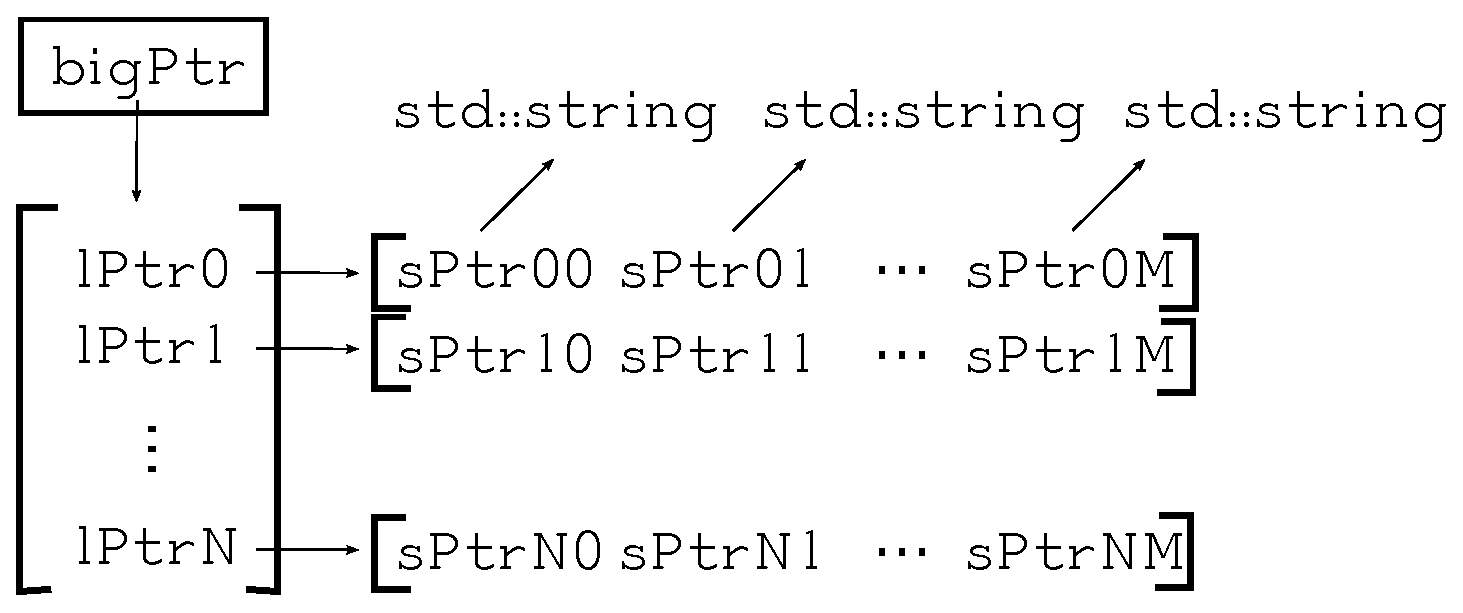
\includegraphics[width=0.5\textwidth]{../48/images/datamodel.eps}
        \caption{\texttt{bigPtr} is a triple pointer. It points to an array of 'line pointers', each of these point to an array of \texttt{std::string} pointers representing the comma-seperated values. For example: using the notation above we have \texttt{bigPtr[1][1] = sPtr11} for the second value on the second line.}
    \end{figure}

    \subsection*{csv.h}
    \cppfile{../48/csv/csv.h}
\end{solution}
